\documentclass{report}
\usepackage{graphicx}
\usepackage[francais]{babel}
\usepackage[utf8]{inputenc}  
%\usepackage[T1]{fontenc}
\usepackage{amsfonts}
\usepackage{hyperref}
\usepackage{color}


\DeclareGraphicsExtensions{.pdf,.jpeg,.png,.ps} 
\graphicspath{{images/}} 

% (1) choose a font that is available as T1
% for example:
\usepackage{lmodern}

% (2) specify encoding
\usepackage[T1]{fontenc}

% (3) load symbol definitions
\usepackage{textcomp}

%-------------------------------------------maths ---------------------------------------------
\usepackage{amsthm}
\newtheorem{mydef}{Definition}
%------------------------------------------- code ---------------------------------------------
\usepackage{minted}
%-----------------------------------------------------------------------------------------------

%-----------------------------------------------------------------------------------------------

\begin{document}
\title{Rapport probabilistic model}
\author{CARRARA Nicolas}
\date{Le 24 juillet 2014}
\tableofcontents

%-----------------------------------------------------------------------------------------------


\part{Introduction}

Ce rapport s'inscrit dans une étude des champs neuronaux dynamiques. Dans ce papier il sera question d'étudier plusieurs routages, c'est à dire les manières de faire communiquer les neurones entre eux. On va ,la plupart du temps, étudier le routage d'un graphe ou d'une superposition de graphe de taille 9x9. En générale un nœud du graphe fera office de neurone et une arrête entre deux nœuds, une synapse.

Jusqu'alors nous travaillions sur le modèle CNFT (ref) . Rappelons tout d'abord en quoi consiste ce modèle. Nous avons un réseau de neurones. Chaque neurone est connecté avec l'ensemble des autres neurones. Chaque neurone dispose d'un seuil d'activation. Après avoir reçu une charge suffisamment importante en tension, le neurone s'active et envoie un spike (une décharge en tension) aux neurones afférents. Cet envoi suit un routage bien particulier : l'idée est d'envoyer des tensions plus faibles aux neurones les plus éloignés en suivant une courbe type différence de deux gaussiennes. Le problème de ce modèle est qu'il requière une interconnexion de neurones globale. Chaque neurone est lié aux autres neurones. Du fait du nombre de connexions,il sera difficile d'implémenter ce routage sur une carte FPGA par exemple. Or c'est notre objectif ici. Un tel modèle pourrait permettre à un robot de faire de la reconnaissance de forme et du suivi de cible.

Afin d'alléger le modèle CNFT dans son ensemble, on va s'intéresser à des type de routage qui ne nécessitent pas autant de connexions neurales. Ce rapport a donc pour objectif d'exposer les différents outils mis à disposition afin de tester différents routages dans le cadre de ce modèle. On va voir comment générer des données relatives à ces routages et comment les analyser. La mise en pratique sera faite avec le routage Probabilistic flooding. Ce routage connecte les neurones seulement voisins de manière 4-connexe. Avant l'envoi d'un spike, le neurone émetteur fait un test de Bernoulli avec un poids particulier (qu'on appellera weigth ou poids par la suite) commun à tous les neurones du modèle, si le test est raté, alors il envoie le spike sinon il le détruit.

Ce rapport résume le travail que réalisé au cour des deux mois d'été ,juillet-août 2014, dans l'équipe Cortex sous la direction de Benoit Chapellet de Vangel et Bernard Girau. Il a été question de développer un framework de simulation pour différents routages puis un framework de test de ces routages. Le framework de simulation est écrit en Java et se greffe au logiciel DNFSim de Benoit Chapellet de Vangel. Il permet de créer,visualiser et analyser un réseau. La conception du framework est telle qu'il est assez générique pour créer tout type de graphe. Dans un second temps, nous nous sommes concentrés sur un framework de test pour ces réseaux. Ce dernier permet de générer un jeu de données produit par DNFSim,d'analyser la répartition des paquets sur ce réseau et de vérifier l'émergence de certaines propriétés du réseau. Afin de valider ce travail et par la même occasion émettre une piste de nouveau routage, on a prit pour exemple le routage Probabilistic flooding qu'on a par la suite intégré au modèle CNFT.

%-----------------------------------------------------------------------------------------------
\part{Network}

Dans cette partie, nous allons présenter le framework de simulation de réseaux ainsi que son application sur plusieurs exemples.

\section{Objectif}

Notre but est de pouvoir concevoir des réseaux de manières génériques et assez intuitives. Le programme se doit d'être évolutif. On s'oriente vers la création d'un framework en java afin de le greffer sur le logiciel DNFSim déjà existant.

\section{Genericité}

Dans l'optique de représenter différents routage, le framework se doit d'être générique. On doit être capable de créer un graphe avec des nœuds et des arêtes avec un comportement particulier. Les informations circulant sur le réseau (paquets) sont eux aussi déclinables sous plusieurs formes. Très succinctement, un réseau est représenté par un \textbf{SpreadingGraph.java} . Ce réseau possède des nœuds \textbf{Node.java} ainsi que des arêtes qui lient ces nœuds. Sur ce réseau circulent des informations sous forme de paquets \textbf{Packet.java} . Toutes ces classes sont paramétrables et déclinables sous des classes filles. Voir la javadoc pour plus d'informations.


\section{Le routage probabilistic flooding}

Le routage probabilistic flooding se base sur la notion de probabilistic flooding à la spécificité près que les nœuds sont liés de manière 4 connexes i.e chaque nœud est lié à son voisin nord, sud, est et ouest. On associe à tous les nœuds un poids commun. Ce poids est utilisé à chaque computation du graphe. Lors d'une computation, le nœud choisit un paquet qu'il possède en file d'attente (FIFO). Il lance alors une expérience de Bernoulli paramétrée par le poids donné. Si il réussit alors il détruit le paquet, si il rate il le laisse passer.
On retrouve toutes les classes relatives à ce routage dans le package main.java.network.probabilisticFlooding

\section{Le modèle probabilistic flooding spike}

Afin de tester l'efficacité du routage probabilistic flooding sur le modèle CNFT, nous avons crée le modèle probabilistic flooding spike (PFS). Rappelons que le modèle CNFT représente une interconnexion de neurones qui envoient deux types de signaux : inhibiteur et excitateur. C'est la différence des deux qui définit quel voltage le neurone reçoit. La propagation de chaque type de signal ressemble à une courbe gaussienne. Distinguons maintenant les deux couches dans ce modèle. Les nœuds qui envoient des signaux excitateurs et les nœuds qui envoient des signaux inhibiteurs. Ces deux couches suivent donc un routage bien particulier. C'est ce routage que l'on va remplacer par le routage probabilistic flooding. Ces deux routages sont paramétrés suite aux tests qu'on a pu faire (en partie grâce au framework de test) afin de copier la répartition gaussienne des routages initiaux.

%-----------------------------------------------------------------------------------------------

\part{Stimulus}

Après la création d'un réseau grâce au framework présenté précédemment, il est possible de paramétrer un certain nombre d'événements sur ce réseau. Ça consistera à envoyer des paquets sur le graphe pendant ses computations.

\section{Objectif}

On peut exciter chacun des nœuds du graphe à différents moments. L'objectif est de voir le comportement du graphe (et du routage associé) selon différents événements. Ces événements sont caractérisés par l'envoi de stimulus, i.e l'ajout de paquets à la file d'attente d'un ou plusieurs nœuds à un ou plusieurs moments de la simulation.

\section{Utilisation}

Le framework pour la programmation d'envoi de stimulus se base sur le format xml. Tous les fichiers de programmation doivent se trouver sous le dossier statistiques/stimulis avec l'extension .stimulis (et non .xml). Cette extension est nécessaire aux fichiers de scripts notamment.

Commençons par un exemple. Admettons que l'on veuille envoyer un paquet de type spike au nœud zéro du graphe à l'instant t=0 :
\\
\inputminted[linenos=true,frame=single,label=asend.stimulis]{xml}{/home/nikolai/Work/Loria2014/dnfsim2/statistiques/stimulis/a_send.stimulis}

On retrouve ici trois balises :
\\
\begin{itemize}
\item <programmation> : On stipule qu'on va commencer un programme d'envoi stimulis. L'attribut "class" est le nom de la class Java des paquets que l'on veut envoyer en tant que stimulis.
\item <time> : Pour spécifier les envois à un temps t donné. A noté que 

\[dtStimulis = k\ *\ dtGraphe\ \forall{k \epsilon{\mathbb{N}^*}}   \] 

i.e on ne peut pas envoyer des stimulis entre deux computations.
\item <add> : On envoie un paquet à l'indice indice. Notez que les indices sont en représentation 1D row-major du graphe.
\end{itemize}

Un exemple d'envoi de paquets ipv4 sur un réseau :\\

\inputminted[linenos=true,frame=single,label=ipv4.stimulis]{xml}{/home/nikolai/Work/Loria2014/dnfsim2/statistiques/stimulis/ipv4.stimulis}

On découvre la balise <params>. L'utilisation de cette balise est directement liée à la structure du constructeur de la classe spécifiée dans la balise programmation. Dans l'exemple précédent on utilisait des spikes, objet simple ne prenant aucun paramètre lors de la construction, on a pas eu besoin d'utiliser la balise <params>. Par contre un paquet ipv4 transporte un message. Ce message est "A". Les valeurs "yes" et "ça fonctionne !" n'ont aucun effet sur la construction d'un objet ipv4 vu qu'il ne prend qu'un string en params.\\

Il faut regarder de plus près le code java.\\



\begin{minted}[linenos=true,frame=single,label=Packet.java]{java}
public class Packet {

    private int size;    
  
    protected Packet(Object ... params){
    }
    
    //...
    
\end{minted}

Chaque classe fille de Packet doit implémenter le constructeur protected.(ça doit être le premier constructeur dans le code pour des raisons d'introspection, même si il y a moyen de faire mieux).\\

\begin{minted}[linenos=true,frame=single,label=Spike.java]{java}
public final class Spike extends Packet {

    public Spike(Object ... params) {
        setSize(1);
    }

}
\end{minted}

On voit que Spike n'utilise aucun de ses paramètres.\\

\begin{minted}[linenos=true,frame=single,label=IPv4Datagramme.java]{java}
public final class IPv4Datagramme extends Packet{
	
	private String message;
	
	public static final int MESSAGE_INDEX = 0;
	
	public IPv4Datagramme(Object ... params) {
        setSize(16); 
        setMessage((String)params[MESSAGE_INDEX]);
	}
	
	//...
\end{minted}

IPv4 utilise un seul paramètre. A noter que les objets récupérés seront de type String.\\


%-----------------------------------------------------------------------------------------------
\part{Génération de données}

\section{Introduction}

Afin de tester certaines propriétés du graphe, il est nécessaire de générer un jeu de données conséquent concernant différentes caractéristiques du routage.

\section{Spikes reçus jusqu'alors}

Dans cette section, nous allons nous intéresser à la génération du jeu de données représentant la quantité de spikes reçus par chaque nœud du graphe, de l'instant 0 à l'instant t.
Pour ce faire, il faut utiliser le script generateData.py.
Ce script s'occupe de lancer cette expérience :\\

\textit{Alice travaille sur le PFModel (probabilistic flooding model), elle envoie des stimulis sur le graphe associé à un ou plusieurs moments de la propagation. Le graphe a une taille et un poids (probabilité de détruire un spike sortant d'un nœud). Alice laisse tourner la propagation pendant t secondes.Elle récupère la matrice représentant le nombre total de spikes reçus par chaque nœuds jusqu'à l'instant t}\\

On lance cette expérience plusieurs fois (itérations) et selon différents paramètres (taille, poids, programmation des stimulis).

Un exemple d'appel de cette commande :
\begin{minted}[frame=single]{python}
python generateData.py --weigths 0.0 0.1 0.2 0.3 0.4 --times 1 2 
--packet_initialisation twoa twob twoab --iterations 100 
--tailles_grilles 9 --forcerewrite
\end{minted}

Ici on génère les données pour les combinaisons de poids temps. On stipule que ce sera de 
taille 9 mais on aurait pu écrire 
\begin{minted}[frame=single]{python} 
--taille_grilles 1 2 3 4 5 6 7
\end{minted}


On veut que l'expérience soit réalisée selon plusieurs programmations (twoa twob et twoab). Les dites programmation doivent se trouver dans le dossier statistiques/stimulis sous la forme nom.stimulis (exemple : twoab.stimulis).

Les données générées se trouvent sous le dossier statistiques/data (avec une arborescence dépendante des paramètres).

A noter que ce script n'est utilisable qu'avec le PFModel pour le moment mais il est facilement extensible à d'autre modèles.\\\\
Faire
\begin{minted}[frame=single]{python}
python generateData.py --help
\end{minted}
pour plus d'informations

%-----------------------------------------------------------------------------------------------

\part{Additivité}

Il est nécessaire de conserver la propriété d'additivité du réseau lors de l'utilisation de nouveaux routages. Pour cela, posons une définition théorique de l'additivité.

\section{Théorie}

A partir de maintenant, on considère un graphe G(N,E) avec N l'ensemble de ses nœuds et E l'ensemble de ses arêtes. Chaque nœud possède une file d'attente FIFO. On peut lancer une propagation sur ce graphe.

\begin{mydef}
(Paquet)
{\color{red}(PAS ASSEZ RIGOUREUX)}

Un \textbf{paquet} $\mathtt{p}$ est un objet. Il contient un certain nombre d'informations. Il se déplace sur le graphe de nœuds en nœuds au fil du temps (lors de la propagation du graphe).
Si le \textbf{paquet} ne contient aucune information, on parle de \textbf{spike}.
\end{mydef}

\begin{mydef}
(Stimulis)

Un \textbf{stimulis} $\mathtt{S}_{p,n,t}$ est le placement du paquet $\mathtt{p}$ dans la file d'attente du nœud n à l'instant t. Si t=0 et si p est un spike, on parle alors d' \textbf{activation}. Une \textbf{activation} $\mathtt{A}_{n}$ est le \textbf{stimulis} $\mathtt{S}_{s,n,0}$
\end{mydef}

\begin{mydef}
(Configuration)

Une \textbf{configuration} $\mathtt{C}$ est un ensemble de stimulis. On parle d'initialisation $\mathtt{I}$ si c'est un ensemble d'activations.
\end{mydef}

\begin{mydef}
(Additivité)

Soit $\mathtt{A^0},\mathtt{A^1}, .. ,\mathtt{A^K}$ des activations où $\mathtt{A^i}=\mathtt{A}_{n_i} \forall i$.

On pose l'initialisation $\mathtt{I}=\{\mathtt{A^k}\ |\ n\epsilon[0,K]\ et\ K>0\}\  $ 

On pose $\mathtt{I}_k = \{\mathtt{A^k}\}\ \forall n\epsilon[0,K]$\\

Soit $M_{t,n,\mathtt{I}}$ la variable aléatoire qui représente l'ensemble des paquets reçus par le nœud n depuis le début de la propagation pour chaque nœud du graphe à l'instant t selon l'initialisation $\mathtt{I}$.\\

On pose $M_{t,\mathtt{I}}=(M_{t,0,\mathtt{I}},M_{t,1,\mathtt{I}},...,M_{t,card(N),\mathtt{I}})$ et $M_{t,\mathtt{I}_i}=(M_{t,0,\mathtt{I}_i},M_{t,1,\mathtt{I}_i},...,M_{t,card(N),\mathtt{I}_i})$ \\

On dit que le routage est \textbf{additif pour l'initialisation} $\mathtt{I}\ si\ \forall t$  

\[\mathbb{E} (M_{t,\mathtt{I}}) = \sum_{i=1}^{n} (\mathbb{E} (M_{t,\mathtt{I}_i})) \]\\

On dit qu'un routage est \textbf{additif} si il l'est pour n'importe quelle initialisation.\\

Note : On pourrait parler d'additivité pour une configuration qui n'utilise que des spikes, et pas forcement une initialisation.
\end{mydef}

\section{Utilisation du script}

Afin de tester cette propriété d'additivité sur des résultats expérimentaux, nous avons crée un script en Scilab. Ce dernier lit un ensemble de donnée de plusieurs répétitions d'expériences afin d'extraire une moyenne de ces données, puis il va calculer à quel point le routage est additif sur ces résultats moyens.


Par exemple 
\begin{minted}[frame=single]{python} 
scilab -nw -f Additivite.sce -args '9' '1 2' 
'0.0 0.1 0.2 0.3 0.4' '5 20 50 75 100' 
'twoa twob' twoab 0 
\end{minted}

vérifie l'additivité twoa+twob=twoab sur les combinaisons possibles entre\\

\begin{itemize}
	\item tailles : 9
	\item times : 1 2 (secondes)
	\item poids : 0.0 0.1 0.2 0.3 0.4
	\item tailles échantillons : 5 20 50 75 100 (nombre de répétition de l'expérience)
\end{itemize}

\section{Résultats}

On veut tester l'additivité dans un milieu épuré. On prend une grille 9x9 de nœuds. On rajoute un spike en haut à gauche(a\textunderscore send) et en bas à droite(b\textunderscore send).On distingue les deux scénarios. On regarde la répartition des spikes au bout de 1,3 et 5s. On fait de même en rajoutant les spikes au deux endroits dès le début (ab\textunderscore send).

On lance la commande suivante : 

\begin{minted}[frame=single]{python} 
scilab -nw -f Additivite.sce -args 
'9' '1 3 5' 
'0.0 0.1 0.2 0.3 0.4 0.5 0.6 0.7 0.8 0.9 1.0' 
'10 50 100 500 1000' 'a_send b_send' ab_send 0
\end{minted} 

On obtient les trois figures suivantes : 

\begin{itemize}
	\item figure~\ref{fig:additivite1s} sur la page~\pageref{fig:additivite1s}.
	\item figure~\ref{fig:additivite3s} sur la page~\pageref{fig:additivite3s}.
	\item figure~\ref{fig:additivite5s} sur la page~\pageref{fig:additivite5s}.
\end{itemize}



\begin{figure}[htbp]
\begin{center}
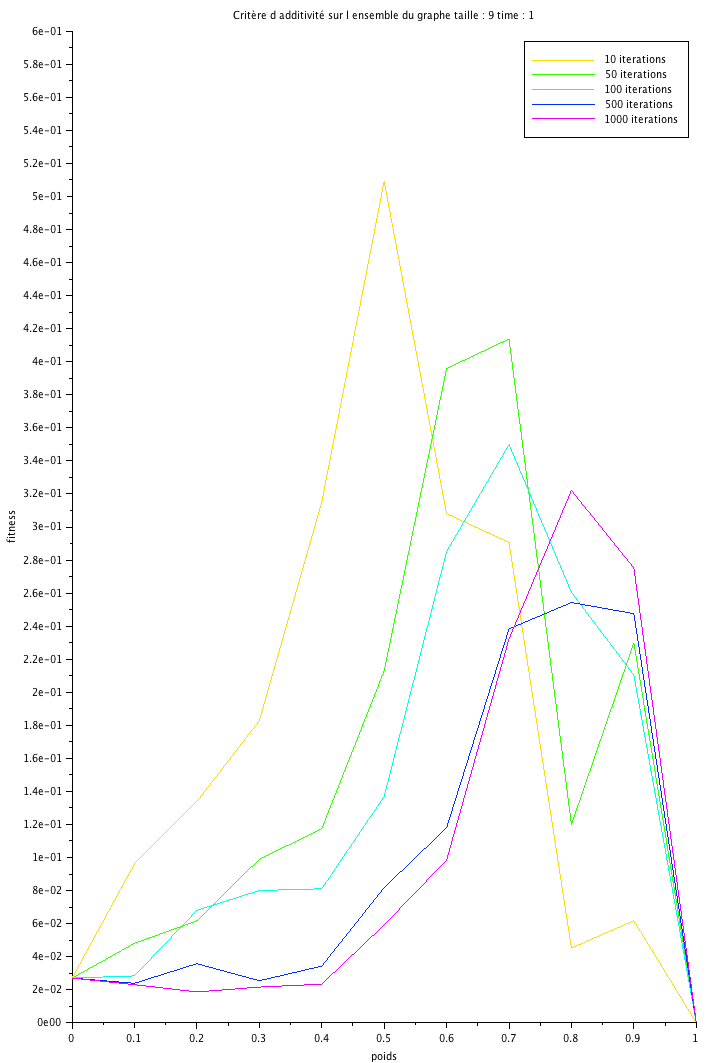
\includegraphics [width=1.0\textwidth]{images/Additivite1s.png}
\caption{Additivité sur l'ensemble du graphe, envoie d'un spike en A, 10 computations}
\label{fig:additivite1s}
\end{center}
\end{figure}

\begin{figure}[htbp]
\begin{center}
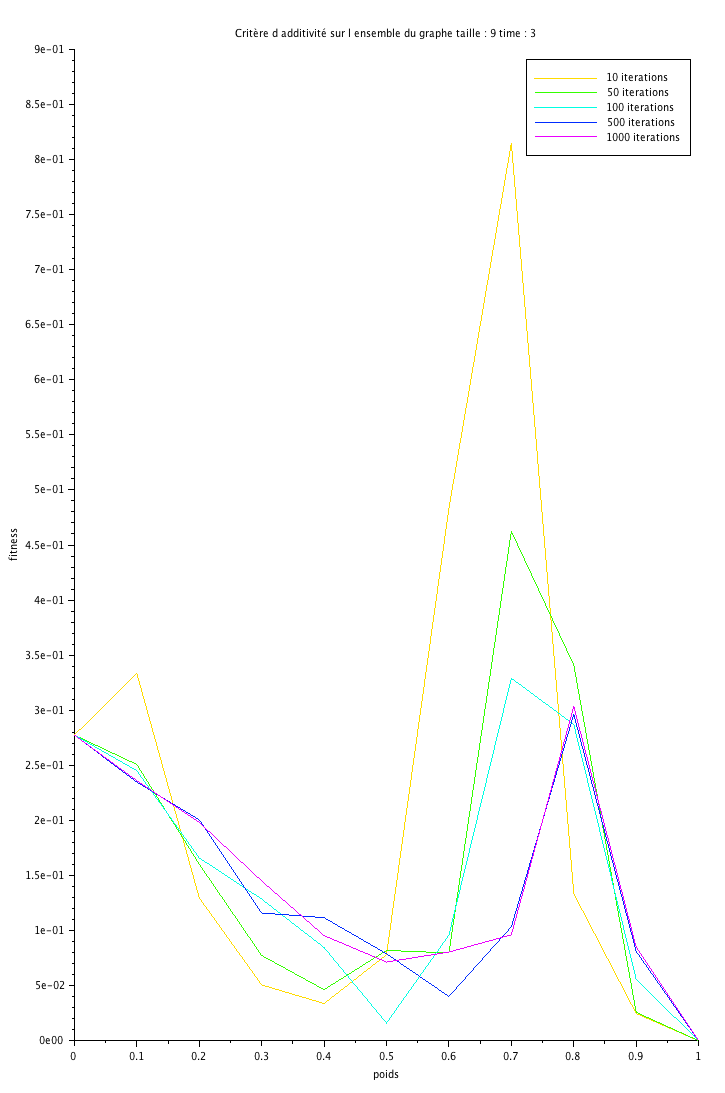
\includegraphics [width=1.0\textwidth]{images/Additivite3s.png}
\caption{Additivité sur l'ensemble du graphe, envoie d'un spike en A, 30 computations}
\label{fig:additivite3s}
\end{center}
\end{figure}

\begin{figure}[htbp]
\begin{center}
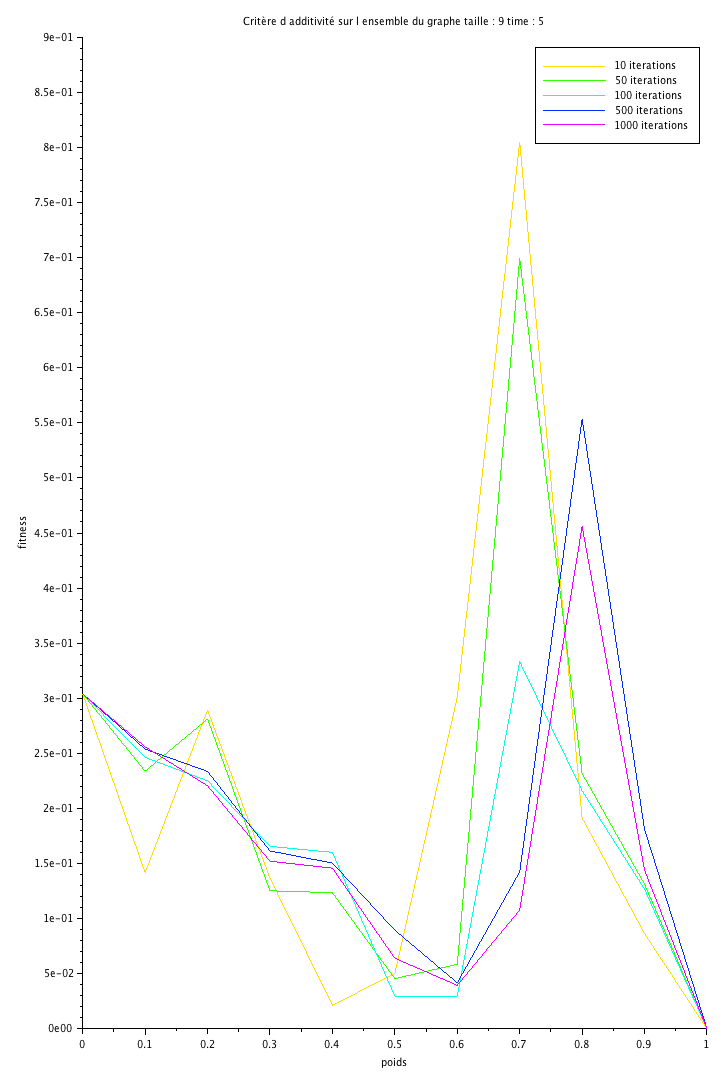
\includegraphics [width=1.0\textwidth]{images/Additivite5s.png}
\caption{Additivité sur l'ensemble du graphe, envoie d'un spike en A, 50 computations}
\label{fig:additivite5s}
\end{center}
\end{figure}

On remarque que l'activité fluctue bien moins quand on augmente le nombre d'expériences. Cette dernière observation pourrait nous amener à la conclusion qu'il faille lancer plusieurs spikes en même temps par activation de neurone (on simulerait en quelque sorte la répétition d'expérience même si on a aucune garantie que le comportement soit similaire. C'est à tester).

On voit un optima autour du poids 0.6 à 5s de computations. Il faudrait voir après 5s de computations. Pourquoi trouve t on une singularité en 0.6 et pas en 0.0 ?

%-----------------------------------------------------------------------------------------------

\part{Propagation des spikes}

Pour qu'un nouveau modèle soit viable, en plus d'avoir un comportement additif, il doit avoir une répartition voltaïque de type "différence de deux gaussienne". Dans cette partie on va voir comment vérifier cette propriété et si notre modèle "Probabilistic flooding" permet d'obtenir la répartition désirée.

\section{Utilisation du script}

Le script MeanAndVariance.sce permet d'obtenir les statistiques moyennes variances et écart type sur un échantillon d'expériences et ce en utilisant différents paramètres. Un exemple de cette commande : 

\begin{minted}[frame=single]{python} 
scilab -nw -f MeanAndVariance.sce -args 
9 '1 3 5' '0.7' 1000 a_send_20 temp/
\end{minted}

avec respectivement comme arguments :

\begin{itemize}
  \item 9 : la taille du réseau (la racine)
  \item '1 3 5' : les temps de computations 
  \item '0.3 0.7' : les poids
  \item 1000 :le nombre d'expériences qu'on utilise pour calculer nos statistiques
  \item a\textunderscore send\textunderscore 20 : le scénario des expériences (a \textunderscore send \textunderscore 20.stimulis doit de trouver sous le dossier stimulis/)
  \item temp/ : le dossier sous lequel les images vont être enregistrées
\end{itemize}

Cette commande va générer sous le dossier temp un ensemble de graphiques représentant les 3 statistiques sur l'ensemble du graphe et sur la diagonale.

\section{Résultats}

On voit sur l'image \ref{fig:moyenne3s07w} de la page~\pageref{fig:moyenne3s07w}. que c'est avec un poids de 0.7 et un temps de computation de 3s qu'on obtient une courbe proche de ce que l'on cherche.

\begin{figure}[htbp]
\begin{center}
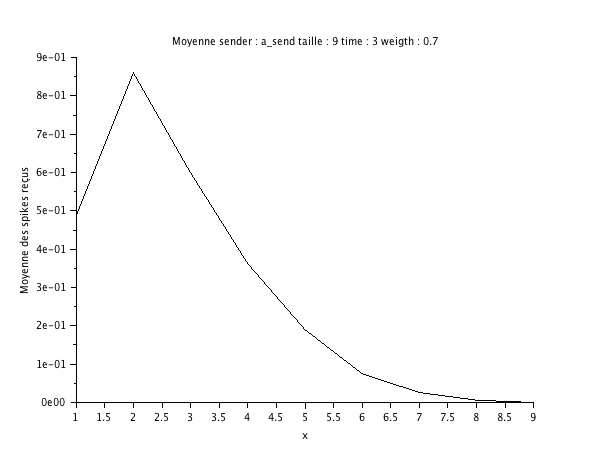
\includegraphics [width=1.0\textwidth]{{images/spike_data_diag1_Moyenne_inita_send_taille9_time3_weigth0.7}.png}
\caption{Répartition des spikes en moyenne sur la diagonale, 30 computations, poids 0.7}
\label{fig:moyenne3s07w}
\end{center}
\end{figure}

Le problème c'est que l'écart type est élevé comme on peut le voir sur l'image ~\ref{fig:ecartmoyenne3s07w} de la page~\pageref{fig:ecartmoyenne3s07w}. 

\begin{figure}[htbp]
\begin{center}
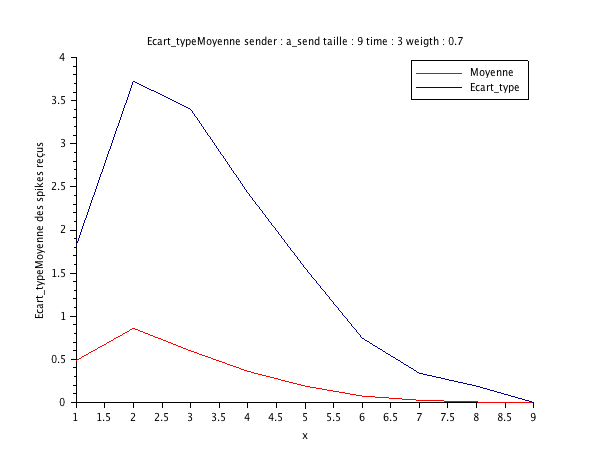
\includegraphics [width=1.0\textwidth]{{images/spike_data_diag1_Ecart_typeMoyenne_inita_send_taille9_time3_weigth0.7}.png}
\caption{Répartition des spikes en moyenne et écart type sur la diagonale, 30 computations, poids 0.7}
\label{fig:ecartmoyenne3s07w}
\end{center}
\end{figure}

\section{Réflexions}

Afin de voir si ce modèle est fiable et pas trop aléatoire on se penche sur le calcul d'un intervalle de confiance autour de la moyenne. Le seul problème c'est que la distribution ne suit pas une loi de probabilité connu, comme on peut le voir sur sur l'image ~\ref{fig:violin} de la page~\pageref{fig:violin}, du coup on pourrait s'orienter vers des méthodes bootstrap.

\begin{figure}[htbp]
\begin{center}
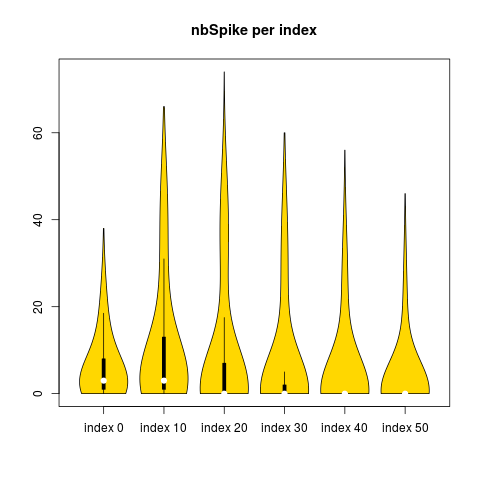
\includegraphics [width=1.0\textwidth]{images/violin.png}
\caption{Violins pour la répartition sur la diagonale}
\label{fig:violin}
\end{center}
\end{figure}

%-----------------------------------------------------------------------------------------------
\part{Probabilistic flooding et I/E}

On rappelle que l'objectif est de trouver un modèle de réseau neuronal simulant le comportement de DNF tout en consommant moins de ressources. Pour cela on va utiliser le routage probabilitic flooding. Ce routage comme vu précédemment s'avère additif et suit une distribution exponentielle/gaussienne selon certains paramètres. On a donc le candidat idéal pour simuler le routage originel de DNF. On va donc mettre en place deux couches de graphes utilisant le routage PF (probabilitic flooding). Une couche avec des signaux excitateurs et une autre avec des signaux inhibiteurs. On applique une transformation affine à ces deux couches puis on soustrait l'une et l'autre. On obtient à la fin la distribution du potentiel des neurones en fonction de leur éloignement aux stimulis. On veut que cette distribution ressemble à la différence de gaussienne du routage de DNF. Pour ça on doit trouver les paramètres des transformations affines ainsi que les poids et les temps de computations des deux graphes. C'est le script InhibiteurExcitateur.sce qui nous permet d'observer l'effet de tel ou tel paramètre sur le comportement voltaïque du réseau de neurones.

\section{Utilisation du script}

Le script InhibiteurExcitateur.sce permet d'observer la répartition voltaïque sur la diagonale d'un réseau de neurones. Comme expliqué précédemment, on superpose deux couches de graphes suivant le routage probabilistic flooding puis on leur applique à chacun une transformation affine. Ce script va afficher la fonction 

\[a_{e} * E(w_{e},t_{e}) + b_{e} - (a_{i} * I(w_{i},t_{i}) + b_{i})\] 

L'interface du script :

\begin{minted}[frame=single]{sh} 
scilab -nw -f InhibiteurExcitateur.sce -args 
taille configuration repetition wi ti ai bi we te ae be
\end{minted}

avec respectivement comme arguments :

\begin{itemize}
  \item taille : la taille du réseau (la racine)
  \item configuration : la configuration (asend, bsend ...)
  \item repetition : le nombre d'expériences qu'on utilise pour calculer nos statistiques
  \item wi : le poids pour le graphe d'inhibition
  \item ti : le temps de computation pour le graphe d'inhibition
  \item ai : le coefficient directeur de la fonction affine du graphe inhibiteur
  \item bi : la constante de la fonction affine du graphe inhibiteur 
  \item we : le poids pour le graphe d'excitation
  \item te : le temps de computation pour le graphe d'excitation
  \item ae : le coefficient directeur de la fonction affine du graphe d'excitation
  \item be : la constante de la fonction affine du graphe d'excitation
\end{itemize}

\section{Résultats}

On veut obtenir une courbe de cette forme : image ~\ref{fig:wantedcurve} de la page~\pageref{fig:wantedcurve} .On lance : 

\begin{figure}[htbp]
\begin{center}
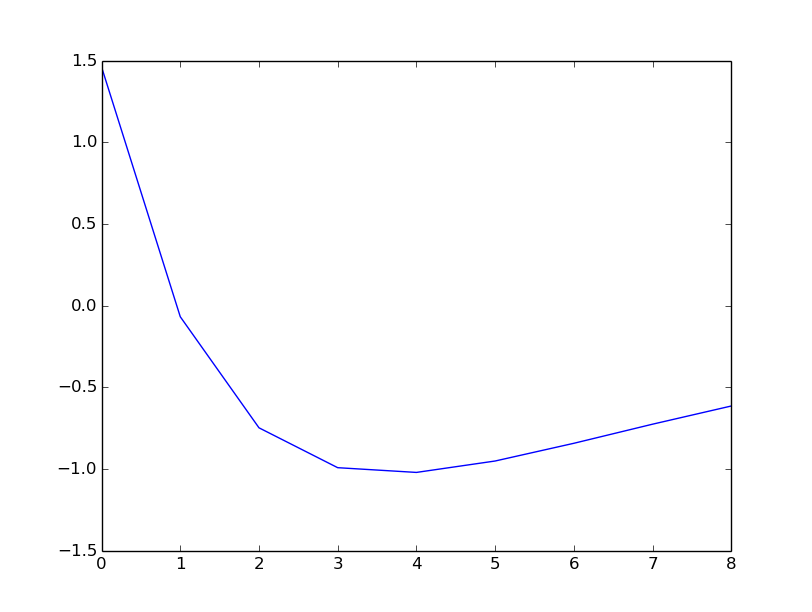
\includegraphics [width=1.0\textwidth]{images/wanted_curve.png}
\caption{Différence théorique de gausiennes }
\label{fig:wantedcurve}
\end{center}
\end{figure}

\begin{minted}[frame=single]{sh} 
scilab -nw -f InhibiteurExcitateur.sce -args 
9 a_send 1000 0.7 7 1.0 0.0 0.7 3.0 4.5 -0.9
\end{minted}

Et on récupère une courbe de cette forme : image ~\ref{fig:wantedcurveexp} de la page~\pageref{fig:wantedcurveexp}. La correspondance nous a semblé suffisante pour des tests en conditions réelles.
\begin{figure}[htbp]
\begin{center}
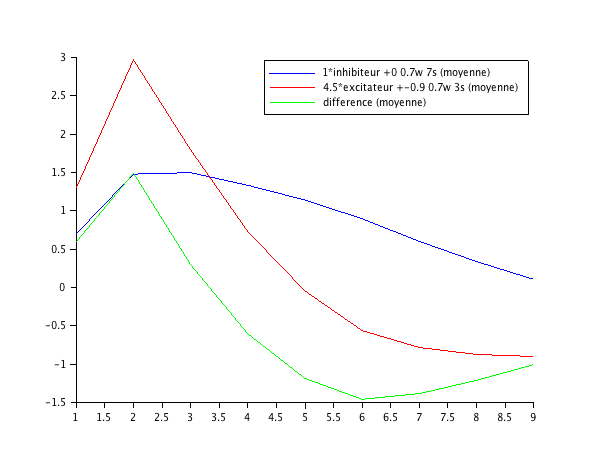
\includegraphics [width=1.0\textwidth]{images/wanted_curve_exp.png}
\caption{Différence expérimentale de gaussiennes}
\label{fig:wantedcurveexp}
\end{center}
\end{figure}

Par contre sur l'image ~\ref{fig:wantedcurveexpvar} de la page~\pageref{fig:wantedcurveexpvar}, on voit déjà un ecart type très élevé de la courbe.

\begin{figure}[htbp]
\begin{center}
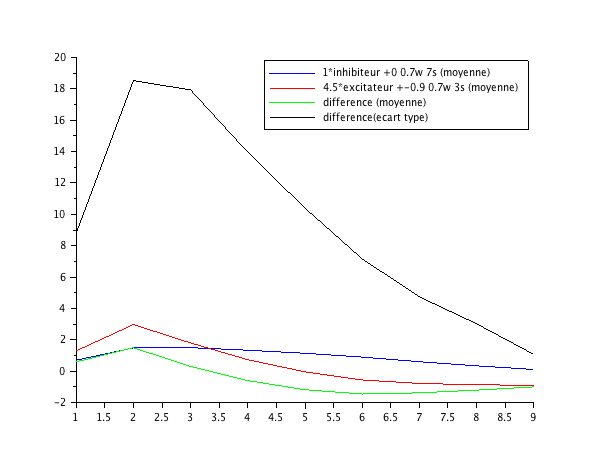
\includegraphics [width=1.0\textwidth]{images/wanted_curve_exp_var.png}
\caption{Différence expérimentale de gaussiennes et écart type de cette différence}
\label{fig:wantedcurveexpvar}
\end{center}
\end{figure}


\section{Application sur dnfsim}

On va donc utiliser cette combinaison linéaire de Probabilistic flooding graphes afin de simuler DNF. Pour cela, on incorpore les différents graphes au logiciel dnfsim. On run un scénario avec deux bulles à des positions opposées qui tournent. Ça fonctionne très mal, la variance est très élevée, on a rarement le focus d'une bulle. De toutes façons on aurait du s'en douter en voyant l'image  ~\ref{fig:wantedcurveexpvar} de la page~\pageref{fig:wantedcurveexpvar}. Pour palier à ce problème de variance, on s'oriente sur l'envoi de {\{20,40,60,80\} spikes par activation de neurone pour voir ce que ça donne. On part de l'idée qu'envoyer plusieurs spikes en même temps permettrait la diminution de variance, en effet c'est comme si on répétait l'expérience plusieurs fois. Afin de voir si notre hypothèse est plausible, on va faire quelques simulations dans cette configuration.

\section{Variance pour \{20,40,60,80\}\textunderscore asend}

On va se placer dans un scénario de test afin de voir si notre hypothèse est plausible et diminue en effet la variance. Pour ça on va supposer que notre scénario de départ permet l'envoi de \{20,40,60,80\} en A (en haut à gauche du réseau). Puis on va observer la répartition des spikes sur la diagonale du réseau (de A à B - en bas à droite - ). On en déduit une variance ainsi qu'un intervalle de confiance pour cette variance.

\subsection{Utilisation du script}

Il suffit de run en ligne de commande. 

\begin{minted}[frame=single]{python} 
scilab -nw -f MultiBootstrap.sce taille weigth time repetition
\end{minted}

avec comme paramètres : 

\begin{itemize}
  \item taille : la taille du réseau (la racine)
  \item repetition : le nombre d'expériences qu'on utilise pour calculer nos statistiques
  \item weigth : le poids pour le graphe
  \item time : le temps de computation (avec dt = 0.1)
\end{itemize}

Ce script affiche la variance selon les configurations 1/20/40/60/80 ainsi que l'intervalle bootstrap à 95%.

\subsection{Résultats}



Afin de voir si on a de meilleurs résultats en terme de variance que les images ~\ref{fig:varw7s3} de la page~\pageref{fig:varw7s3} et ~\ref{fig:varw7s7} de la page~\pageref{fig:varw7s7}

\begin{figure}[htbp]
\begin{center}
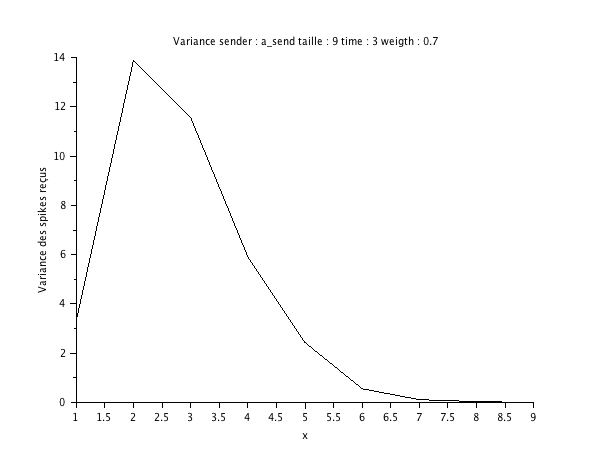
\includegraphics [width=1.0\textwidth]{{images/spike_data_diag1_Variance_inita_send_taille9_time3_weigth0.7}.png}
\caption{Variance de la répartition des spikes sur la diagonale lors de l'envoi d'un stimulis en A. 30 computations, poids 0.7.}
\label{fig:varw7s3}
\end{center}
\end{figure}


\begin{figure}[htbp]
\begin{center}
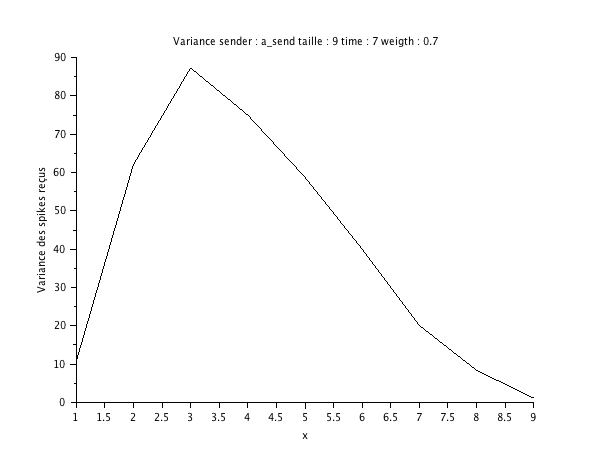
\includegraphics [width=1.0\textwidth]{{images/spike_data_diag1_Variance_inita_send_taille9_time7_weigth0.7}.png}
\caption{Variance de la répartition des spikes sur la diagonale lors de l'envoi d'un stimulis en A. 70 computations, poids 0.7.}
\label{fig:varw7s7}
\end{center}
\end{figure}

On lance 

\begin{minted}[frame=single]{python} 
scilab -nw -f MultiBootstrap.sce 9 0.7 3 1000
\end{minted}

et 

\begin{minted}[frame=single]{python} 
scilab -nw -f MultiBootstrap.sce 9 0.7 7 1000
\end{minted}

Voici les résultats : 

\begin{itemize}
  \item ~\ref{fig:varallw7t3} de la page~\pageref{fig:varallw7t3}
  \item ~\ref{fig:varbootallw7t3} de la page~\pageref{fig:varbootallw7t3}
  \item ~\ref{fig:varallw7t7} de la page~\pageref{fig:varallw7t7}
  \item ~\ref{fig:varbootallw7t7} de la page~\pageref{fig:varbootallw7t7}
\end{itemize}


\begin{figure}[htbp]
\begin{center}
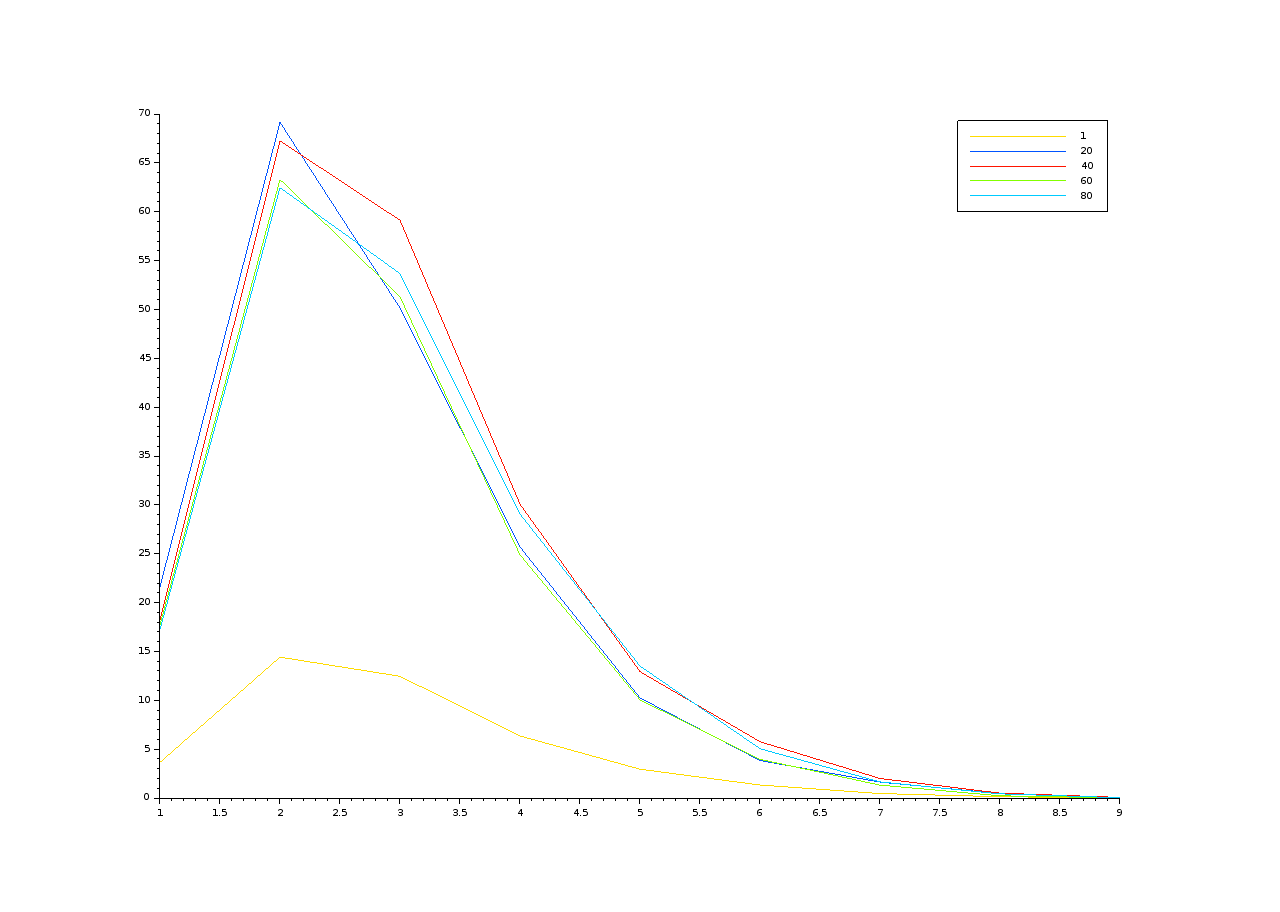
\includegraphics [width=1.0\textwidth]{images/variance120406080send.png}
\caption{Variances de la répartition des spikes sur la diagonales pour 1/20/40/60/80 envois de spikes en A. 30 computations, poids 0.7.}
\label{fig:varallw7t3}
\end{center}
\end{figure}
\begin{figure}[htbp]
\begin{center}
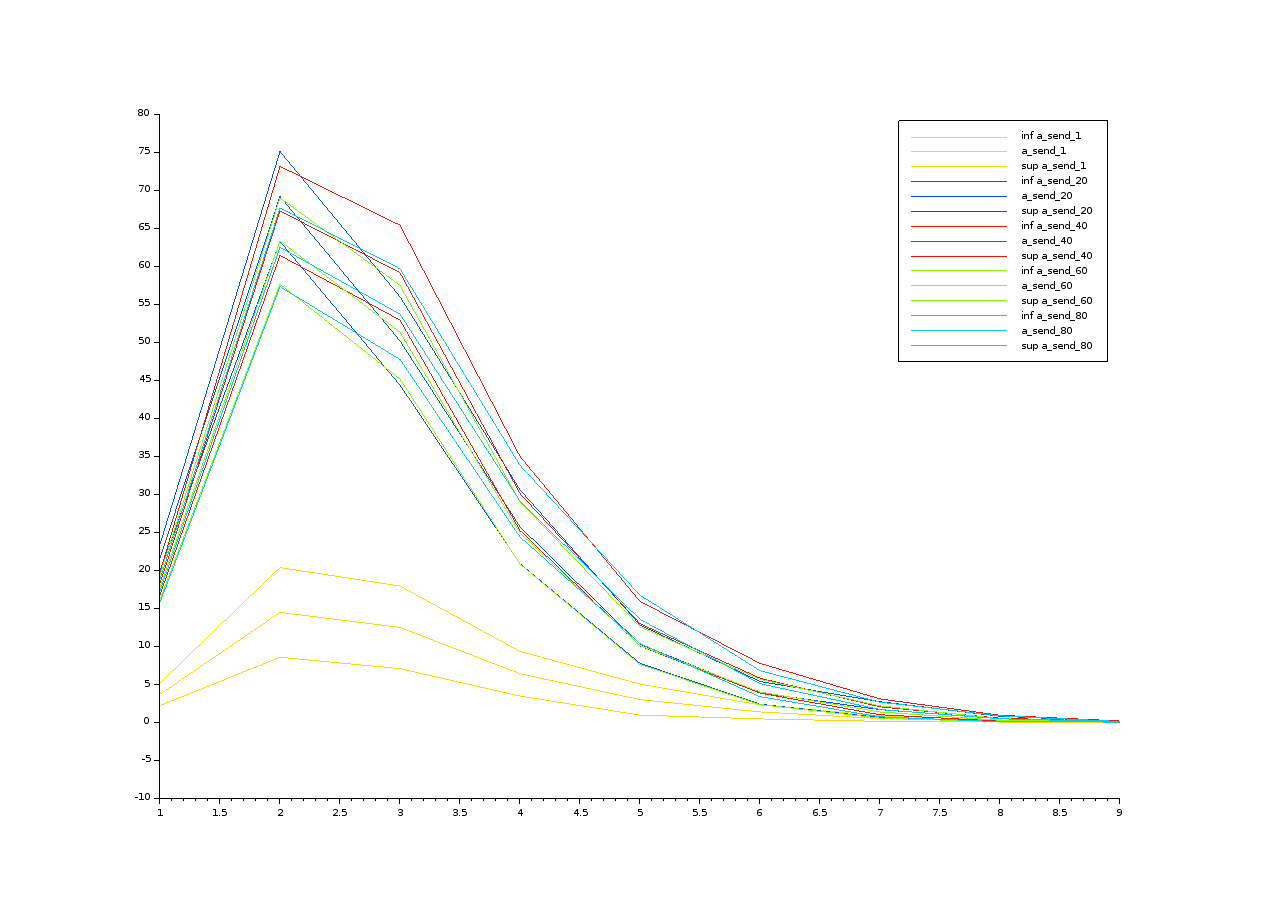
\includegraphics [width=1.0\textwidth]{images/variancebootstrap120406080send.png}
\caption{Variances (et son intervalle de confiance) de la répartition des spikes sur la diagonales pour 1/20/40/60/80 envois de spikes en A. 30 computations, poids 0.7.}
\label{fig:varbootallw7t3}
\end{center}
\end{figure}
\begin{figure}[htbp]
\begin{center}
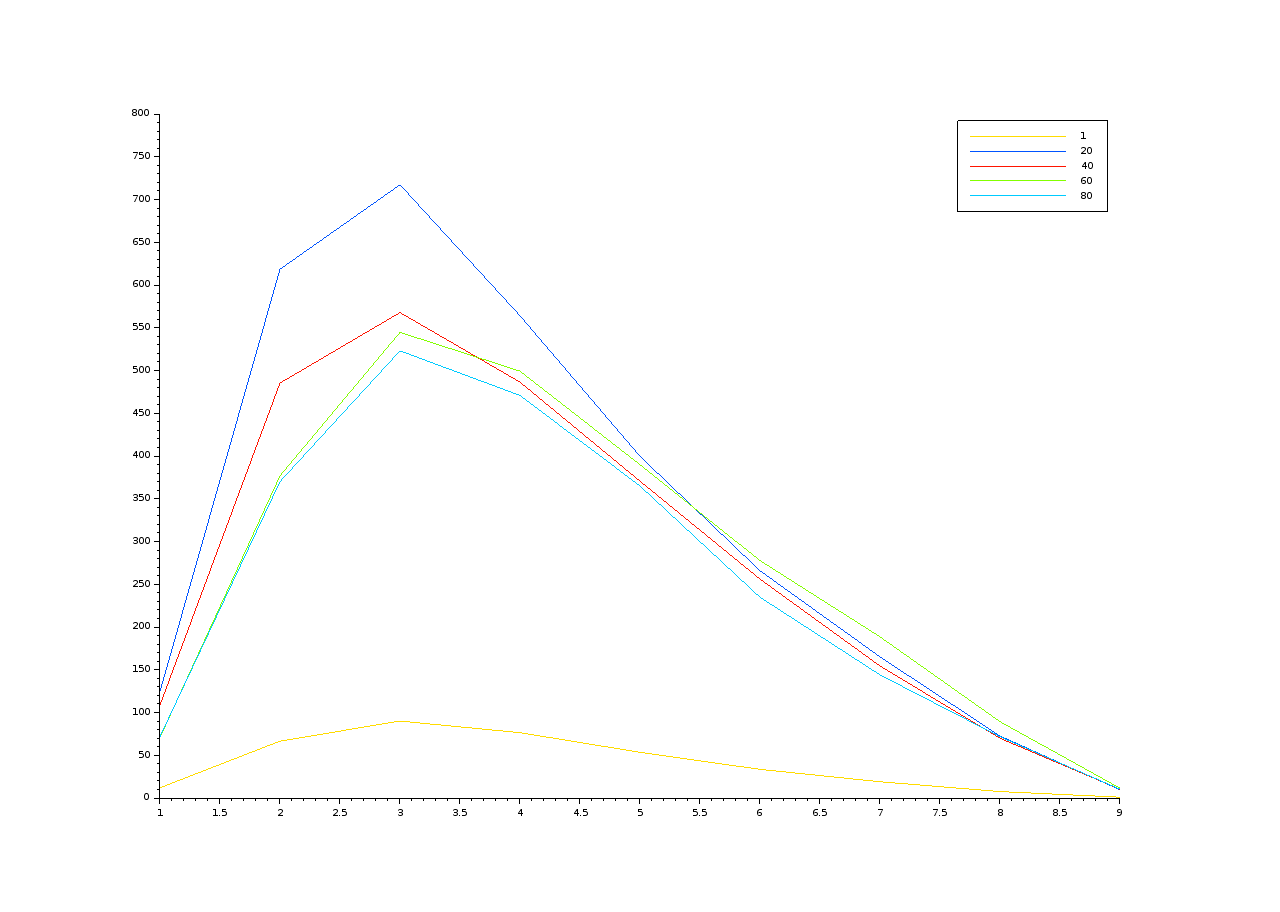
\includegraphics [width=1.0\textwidth]{images/variance120406080sendbis.png}
\caption{Variances de la répartition des spikes sur la diagonales pour 1/20/40/60/80 envois de spikes en A. 70 computations, poids 0.7.}
\label{fig:varallw7t7}
\end{center}
\end{figure}
\begin{figure}[htbp]
\begin{center}
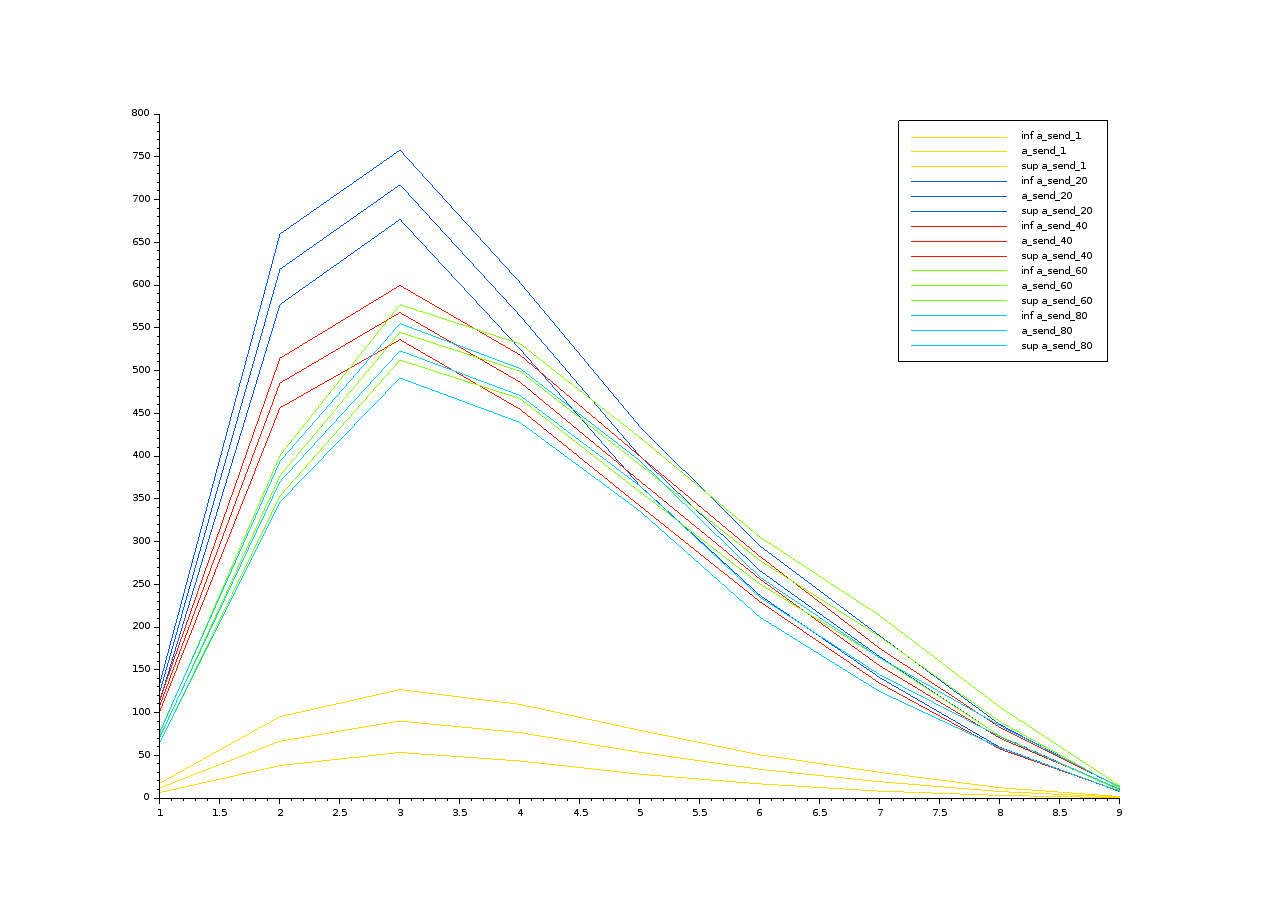
\includegraphics [width=1.0\textwidth]{images/variancebootstrap120406080sendbis.png}
\caption{Variances (et son intervalle de confiance) de la répartition des spikes sur la diagonales pour 1/20/40/60/80 envois de spikes en A. 70 computations, poids 0.7.}
\label{fig:varbootallw7t7}
\end{center}
\end{figure}



Comme on peut le constater, notre hypothèse se révèle être complètement fausse, on a beaucoup plus de variance en multipliant les spikes à l'origine. (problème de programmation ?) . A mon avis c'est normal. La variance est plus élevée car la moyenne est plus élevée. Il faudrait calculer la variance sur la même variable aléatoire (nombre de spikes reçus sur la diagonale) mais divisée par le nombre de spikes envoyés. Par contre, ça n'expliquerait pas pourquoi les variances avec 20/40/60/80 spikes sont similaires.

On a quelques pistes pour diminuer la variance du routage : 

\begin{itemize}
	\item wrapper les maps 
	\item connexion 8-connexe
	\item superposer plusieurs maps E et plusieurs map I et faire la moyenne
	\item rendre certain le transfert des spike aux quatre premiers voisins
	\item rendre des connexions obsolètes après une ou deux computations suite au transfert d'un spike

\end{itemize}
 
%-----------------------------------------------------------------------------------------------
\part{TODO}

\begin{itemize}
	\item expliquer les résultats pour avoir une meilleur compréhension des paramètres
	\item g1 additif,g2 additif => a*g1+b*g2+c additif ?
	\item tous les scripts scilab travaillent avec le dossier toric\textunderscore F, faire en sorte de choisir entre toric et non toric.
\end{itemize}

\end{document}
